
\subsubsection{Thermal Treatment}
When two sufficiently flat and smooth glass surfaces are brought into contact,
the direct bonding process initiates. One of the first mechanisms to occur is
the formation of hydrogen bonds. These bonds can subsequently be transformed
into stronger covalent bonds, as described by the following chemical reaction:
\begin{equation}
\mathrm{Si-OH + HO-Si} \rightleftharpoons \mathrm{Si-O-Si + H_2O}.
\label{eq:polimer siloxane}
\end{equation}
To achieve permanent covalent bonding, water must be removed from the interface,
rendering the aforementioned reaction irreversible \cite{rammhandbook}. This is
accomplished through a thermal treatment known as \textit{annealing}.
\\\\
Annealing involves baking the bonded components in a controlled environment. The
primary parameters influencing the outcome are the temperature ramp, the
equilibrium temperature, and the annealing time. 
\\\\
The \textit{temperature ramp} refers to the heating rate within the oven.
This gradient should be kept as low as possible, as rapid temperature increases
can induce thermal stress in the glass substrates. Such stress may compromise
mechanical and optical performance, or even result in substrate fracture. 
\\\\
Regarding \textit{equilibrium temperatures}, higher values facilitate greater
water diffusivity, thereby removing moisture from the interface more rapidly.
Furthermore, increased viscous flow enhances surface contact \cite{rammhandbook}.
However, high temperatures are often unsuitable for precision optics,
as they may damage optical coatings or integrated electronics \cite{li2013}. 
In such cases, plasma activation is essential, as it increases surface energy
and water diffusivity at significantly lower temperatures \cite{cho2001}. 
This approach is referred to as \textit{Low-Temperature Direct Bonding}.
\\\\
Concerning \textit{annealing times}, literature indicates that bonding energy
increases monotonically over time, whether through a dedicated annealing process
or by leaving surfaces in contact at room temperature. The relationship between
bonding energy and time follows a logarithmic trend:
\begin{equation}
\gamma \propto \ln\left(\frac{t}{\mu}\right),
\end{equation}
where $t$ is the annealing time and $\mu$ represents a time constant.
The role of annealing is effectively to decrease this $\mu$ constant, 
allowing maximum bonding energy to be
reached much faster. Typical annealing times for optical applications 
range from 2 to 24 hours \cite{cho2001, yu2023, li2013, possl1998,trinh2022}.
An example of how the bonding energy evolves with time can be seen in Figure 
\ref{fig:annealing_time}.
\begin{figure}[h]
\centering
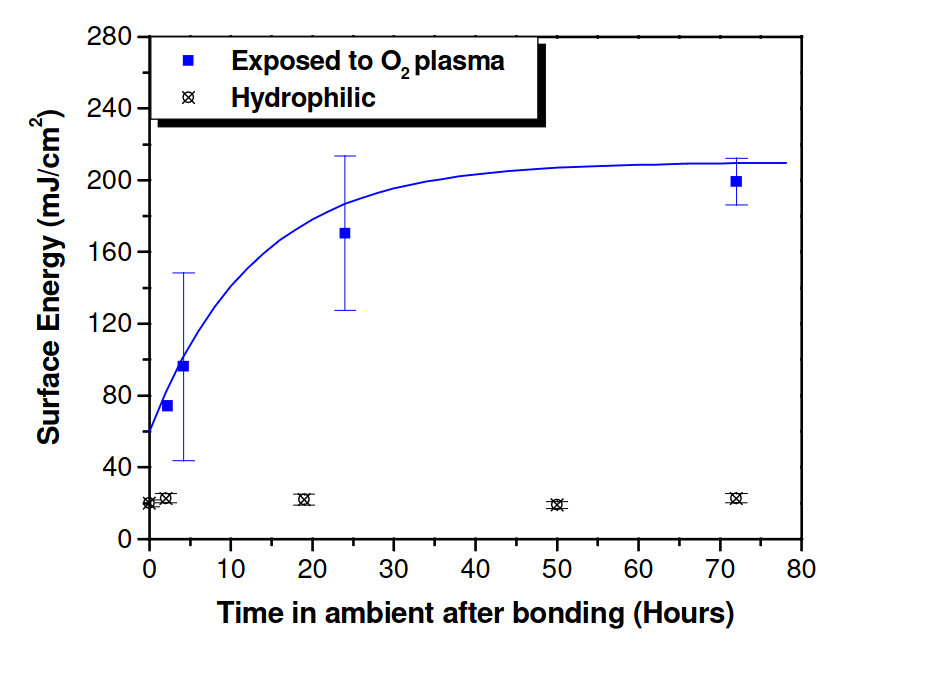
\includegraphics[width=0.8\linewidth]{Images/annealing_time.png}
\caption{Bonding energy evolution with time. From \cite{cho2001}}
\label{fig:annealing_time}
\end{figure}   
